
%(BEGIN_QUESTION)
% Copyright 2006, Tony R. Kuphaldt, released under the Creative Commons Attribution License (v 1.0)
% This means you may do almost anything with this work of mine, so long as you give me proper credit

Følgende kraftbalansemekanisme reagerer på en påført kraft ved å øke utgangstrykket:

$$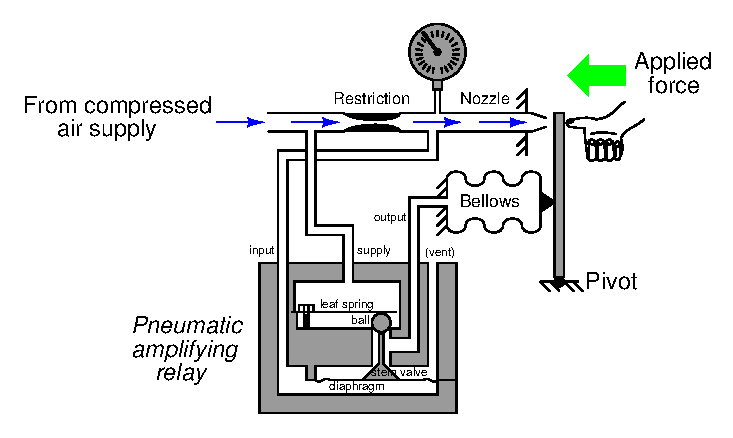
\includegraphics[width=15.5cm]{i00798x01.eps}$$

Hvordan vil denne mekanismen reagere når nøyaktig samme manuelle kraft påføres {\it lavere}, altså nærmere vippepunktet?

$$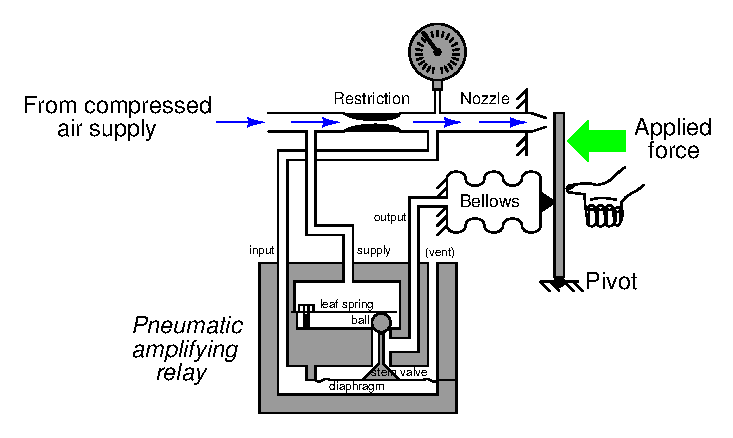
\includegraphics[width=15.5cm]{i00798x02.eps}$$

Forklar {\it hvorfor} dette skjer.

\underbar{file i00798}
%(END_QUESTION)





%(BEGIN_ANSWER)

Utgangstrykket vil ikke øke like mye når samme kraft påføres et punkt nærmere vippepunktet.

%(END_ANSWER)





%(BEGIN_NOTES)

%INDEX% Basics, pneumatics: force-balance mechanism

%(END_NOTES)
